\chapter{導入}

この集中講義ではPCP定理と呼ばれる計算量理論の基本的な結果について解説し, その証明を与える.
PCP定理は1998年に\citet{AroraS98,AroraLMSS98}によって証明された.
この証明は代数的な手法に基づく誤り訂正符号を技巧的に組合せたものであり, 難解なものであったが, その後\citet{Din07}によってより簡潔な証明が与えられた.
この講義では\citet{Din07}による比較的簡単な証明を紹介する.
ちなみにDinurはのちにこの業績によりゲーデル賞を受賞している.

\section{計算量理論の復習}
まずは計算量理論のどの教科書にも載っているような基礎的な用語の定義を与える. これらの用語に明るい読者は\cref{sec:PCP}から読み始めても良い.
なお, このノートではアルゴリズムの定義 (チューリング機械の定義) は省略し, アルゴリズムについて述べる際は具体的な計算の手続きを述べる\footnote{ひとまずPythonやC言語などで実装されたプログラムを考えれば良い. ただし, 計算機内では全ての数値は有限桁の二進数で表記されており, その読み書きや演算には少なくとも桁数に比例した計算時間がかかる. なお, $\sqrt{2}$といった無理数は本来は有限桁で打ち切った近似値を扱うが, そのような小数はこの講義では扱わず, 特に断りのない限りは整数値のみを考える. また, 記憶領域へのアクセスは定数時間で行えると仮定する(チューリング機械であればテープの移動にかかる時間も考慮する).}.

まずは基本的な記号の定義を与える:
\begin{itemize}
\item オーダー記法: 二つの関数$f,g\colon\Nat\to\Nat$に対し, $f(n)=O(g(n))$であるとは, ある定数$c>0$が存在して, 十分大きな全ての$n\in\Nat$に対して$f(n)\le cg(n)$が成り立つことをいう. また, $f(n)=\Omega(g(n)), f(n)=o(g(n)), f(n)=\omega(g(n))$なども同様に($n\to\infty$として)定義する.
\item 自然数$n\in\Nat$に対して$[n]=\qty{1,\dots,n}$とする.
\item 有限集合$S$に対し, $x\sim S$と書いたとき, $x$は$S$から一様ランダムに選ばれた元であることを意味する.
\item 集合$S$上のベクトル$x\in S^n$および$I\subseteq[n]$に対し, $x_I \in S^I$を, $x$の$I$への制限, すなわち, $x_I(i)=x(i)$ ($i\in I$) と定義する.
\item 本資料で登場する全ての有限集合$S=\{s_1,\dots,s_m\}$に対し$s_1<s_2<\dots<s_m$という順序が暗に定まっているとする. 非空な部分集合$T=\qty{t_1,\dots,t_k}\subseteq S$を考える際は常にこの順序に従って$t_1<\dots<t_k$を仮定する. 例えばグラフの頂点集合にも順序が一つ決まっており, 無向辺$e=\{u,v\}$を考える際も\emph{常に}$u<v$を仮定する.
\item $\binset^*=\bigcup_{n\in\Nat}\binset^n$を有限長の二進文字列全体とする.
\item $x\in\binset^*$に対して$\abs{x}$を$x$の文字数とする.
\item アルゴリズム$A$に対し, $A(x)$を入力$x \in \binset^*$に対するアルゴリズム$A$の出力とする. ここで, 単に「アルゴリズム」と言った場合は決定的アルゴリズムを指し, 乱択アルゴリズムについては明示的に言及する.
\item 関数$T(n)\colon\Nat\to\Nat$を考える. 十分大きな全ての$n\in\Nat$と全ての$x\in\binset^n$に対して, $A$が$A(x)$を出力するまでにかかる計算ステップ数の最大値が高々$T(n)$であるとき, アルゴリズム$A$の計算量は$T(n)$であるという. 特に, ある($n$に依らない)定数$c>0$が存在して計算量が$O(n^c)$で抑えられるアルゴリズムを\emph{多項式時間アルゴリズム}という\footnote{計算モデルによって一つ一つの計算ステップの定義は異なるが, 原理的には1bitの演算や記憶領域への読み書きの回数と思えばよい. 多項式時間で動くかどうかの議論であれば, 多くの古典的な計算モデルは等価である.}
\item 計算量理論において慣例的に用いられる記法だが, 関数$f(n)$が$n$に関する多項式である, すなわち$n$に依存しないある定数$c>0$に対して$f(n)=O(n^c)$が成り立つことを$f(n)=n^{O(1)}$または$f(n)=\poly(n)$と表す. 例えば多項式時間アルゴリズムとは, 十分大きな全ての$n\in\Nat$に対して, 長さ$n$の任意の文字列$x\in\binset^n$を受け取ったときの時間計算量が$n^{O(1)}$で抑えられるアルゴリズムである.
\item 二つの文字列$x,y\in\binset^*$を入力として受け取るアルゴリズムは$A(x,y)$と表す. 三つ以上の場合も$A(x,y,z)$などと表す.
\end{itemize}

計算量理論で最も基本的な問題群として判定問題と呼ばれる問題群がある.

\begin{definition}{判定問題}{decision-problem}
  部分集合$L\subseteq\binset^*$を\emph{判定問題(または言語)}といい,
  アルゴリズムに与える$L$の入力を\emph{インスタンス}という.
  また, インスタンス$x\in\binset^*$は$x\in L$であるとき, 判定問題$L$の\emph{Yesインスタンス}といい,
  そうでない場合は\emph{Noインスタンス}という.

  文字列$x\in\binset^*$に対し$L(x)\in\binset$を, $x\in L$かどうかの指示関数, すなわち$x\in L$ならば$L(x)=1$, そうでなければ$L(x)=0$と定義する.

  アルゴリズム$A$は, 任意の$x\in\binset^*$に対して$A(x)=L(x)$が成り立つとき,
  $A$は$L$を解くという.
\end{definition}

\begin{example}{グラフ連結性判定問題}{graph-connectivity-problem}
  グラフ$G=(V,E)$の隣接行列を$A \in \binset^{|V|\times|V|}$とする.
  この行列を長さ$|V|^2$の二進文字列として表現したものを$\mathsf{str}(A)$とする.
  すなわち, $\mathsf{str}(A)$の第$k$ビットは, $i=\ceil{k/|V|}+1, j=k\mod |V|+1$に対して$A(i,j)$の値として与えられる.
  このとき,
  \begin{align*}
    L = \qty{ \mathsf{str}(A)\in\binset^{|V|^2} \colon \text{$A$は連結グラフ$G$の隣接行列} }
  \end{align*}
  は与えられたグラフが連結であるかどうかを判定する判定問題である.
\end{example}

この講義では「効率的に解ける」といった場合, 多項式時間アルゴリズムによって解けることを指す. そのような判定問題の集合をクラスPという.
\begin{definition}{クラスP}{classP}
  判定問題$L$は, それを解く多項式時間アルゴリズムが存在するとき, $\P$に属するといい, $L \in \P$と表す.
\end{definition}

\begin{remark}{入力のフォーマット}{input-format}
  \cref{ex:graph-connectivity-problem}では入力としてグラフの隣接行列を二進文字列として表現したものを考えたが, 一般にグラフの表現方法は他にも隣接リストなどが考えられる.
  しかし, 例えばグラフを隣接行列で表現するか隣接リストで表現するかは, それぞれのフォーマット間の変換が多項式時間で行えるため, \emph{多項式時間で解けるかどうか}という点では等価である.

  そのため, 厳密には問題を定義する際はその入力のフォーマット(グラフを隣接行列で表現するか, 隣接リストで表現するか, など)も指定する必要があるが,
  フォーマット間の変換が自明に多項式時間で行える場合に限ってはこの講義ではそのようなフォーマットの指定を省略し, 例えばグラフ連結性判定問題を「グラフが与えられたときにそれが連結であるかどうかを判定する問題」と表現する.
\end{remark}

次に乱択アルゴリズムについて定義する. 端的に言えばアルゴリズムの内部でコイントスを行うものを乱択アルゴリズムという.
ここでは明示的にランダムシードを受け取るアルゴリズムを乱択アルゴリズムと呼ぶことにする.

\begin{definition}{乱択アルゴリズム}{randomized-algorithm}
  入力$x\in\binset^*$とは別にランダムシード(乱数表)と呼ばれる別の文字列$s\in\binset^*$を受け取るアルゴリズムを\emph{乱択アルゴリズム}といい, ランダムシードであることを強調するために$A(x;s)$などと表す.
  なお, 任意の$x,s\in\binset^*$に対して$A(x;s)$は有限時間で停止するとし, その計算量は$\abs{x}$のみに依存する関数で表せるとする.
  このとき, ランダムシード$s$の長さを常に$A$の計算量で上から抑える.
  すなわち, $A$の計算量が$T(n)$であるとき, 十分大きな全ての$n\in\Nat$と全ての$x\in\binset^n$に対して$A$が読み込む$s$の文字数は高々$T(n)$であるため, $s\in \binset^{T(n)}$であると仮定する.
  しばし, ランダムシード$s$を明記する必要が特にない場合は$A(x)$と表す.

  乱択アルゴリズムのランダムシードに関する確率, 期待値, 分散を議論する際は記号として$\Pr_{A}[\cdot],\E_A[\cdot],\Var_A[\cdot]$を用いる.
  乱択アルゴリズム$A$が判定問題$L$を解くとは,
  \begin{align*}
    \Pr_A[A(x)=L(x)]\geq 2/3
  \end{align*}
  が成り立つことをいう.
\end{definition}

また, 入力とは別に文字列へのオラクルアクセスを受け取るアルゴリズムを考える.
\begin{definition}{オラクルアルゴリズム}{oracle-algorithm}
  文字列$\pi\in\binset^*$に対し, $\pi$への\emph{オラクルアクセス}を持つアルゴリズム$A^\pi(x)$とは, 計算途中で$\pi$の指定された位置の文字を読むことができるアルゴリズムである.
  すなわち, $\pi$の$i$番目の文字を読む操作を$A^\pi(x)$の計算過程中に$O(\log \abs{\pi})$時間で行うことができるアルゴリズムである.\footnote{自然数$i\in[\abs{\pi}]$を指定するために$O(\log \abs{\pi})$ビットを定めなければならないため, $O(\log \abs{\pi})$時間を仮定している.}
  同様に乱択オラクルアルゴリズムについても定義できる.
\end{definition}


\section{検証の計算量}
数学全般における検証とは, ある命題が真であると主張する証明が与えられたとき, その証明が実際に
その命題を正しく証明しているかどうかを確認することを意味する.
論文や記述試験の証明の査読や採点をイメージしてもらうとわかりやすいだろう.
計算量理論では検証やその計算量の議論は重要な研究テーマであり, その検証に要する計算量が議論される.

\subsection{効率的な検証とクラスNP}
判定問題$L$と入力$x\in\binset^*$を与えられたとき, $x\in L$かどうかを審議したい.
ここで$x\in L$を主張する証明が文字列$\pi\in\binset^*$で与えられたとする.
このとき, \emph{検証者}と呼ばれるアルゴリズムは$x$と$\pi$を読み込んで$x\in L$かどうかを判定する.
この判定を多項式時間で行えるとき, その判定問題$L$の集合を$\NP$という.

\begin{definition}{クラスNP}{classNP}
  判定問題$L$は, 以下を満たす多項式時間アルゴリズム$V$と多項式$p\colon\Nat\to\Nat$が存在するとき, $L$は$\NP$に属するという:
  アルゴリズム$V$は入力として$x,\pi\in\binset^*$を受け取り, $0$または$1$を出力する.
  \begin{enumerate}
  \item もし$x\in L$ならば, ある$\pi\in\binset^{p(\abs{x})}$が存在して$V(x,\pi)=1$となる.
  \item もし$x\notin L$ならば, 全ての$\pi\in\binset^{p(\abs{x})}$に対して$V(x,\pi)=0$となる.
  \end{enumerate}
  また, このようなアルゴリズム$V$を\emph{NP検証者}といい, $\pi$を\emph{NP証明}という.
\end{definition}

\begin{remark}{クラスPとNPの関係}{remark.P-NP}
  判定問題$L$が$\P$に属するならば$L\in\NP$である.
  実際, 受け取った$x\in\binset^*$に対して$L(x)$を計算してそれを出力する検証者を考えばよい.
  すなわち$\P\subseteq\NP$である.
  一方, 逆側の包含関係$\NP\subseteq\P$が成り立つかどうかはP vs NP問題と呼ばれる計算量理論における最も重要な未解決問題であり, 多くの研究者は$\NP\subseteq\P$が成り立たないと信じている.
\end{remark}

検証者$V(x,\pi)$が$1$を出力したとき, $V$は証明$\pi$を\emph{受理する}といい,
検証者が$0$を出力したとき, $V$は証明$\pi$を\emph{拒否する}という.

\begin{example}{合成数判定問題}{composite-number-problem}
  判定問題$L=\{x\in\binset^*\colon x\text{は合成数}\}$を考える.
  このとき, 検証者は$x$と$\pi$を読み込んで, $\pi\not\in\{1,x\}$かつ$\pi$が$x$を割り切るかどうかを判定する.
  もしも$x\in L$である場合, 合成数なので非自明な約数を証明$\pi$として与えれば$V(x,\pi)=1$となる.
  そうでない場合, 非自明な約数は存在しないため必ず$V(x,\pi)=0$となる.
  このアルゴリズム$V$は入力長(つまり数値の二進表現したときのビット長)に関する多項式時間で動作するため, $L$はNPに属する.
\end{example}

\begin{example}{グラフ彩色問題}{graph-coloring-problem}
  自然数$k\ge 2$とグラフ$G=(V,E)$に対し, 関数$c\colon V\to[k]$が
  全ての辺$\{u,v\}\in E$に対して$c(u)\neq c(v)$を満たすとき, $c$を$G$の$k$-彩色といい,
  $k$-彩色が存在するようなグラフは$k$-彩色可能であるという.
  任意の$k\ge 2$に対し, 判定問題
  $$L=\{G\in\binset^*\colon G\text{は}k\text{-彩色可能}\}$$
  はNPに属する.
  検証者は$G$と$\pi$を読み込んで, $\pi$が$G$の$k$-彩色であるかどうかを判定する.
  もしも$G\in L$である場合, $G$は$k$-彩色可能であるため, $k$-彩色の証明$\pi$を与えれば$V(G,\pi)=1$となる.
  そうでない場合, $G$は$k$-彩色可能でないため必ず$V(G,\pi)=0$となる.
  このアルゴリズム$V$は多項式時間で動作するため, $L$はNPに属する.
\end{example}

\begin{exercise}{素数判定問題}{exer.prime-problem}
  自然数$n\in\Nat$に対しその二進表記を$(n)_2\in\binset^*$と表す.
  判定問題$\PRIMES=\{(a)_2\in\Nat\colon a\text{は素数}\}$を考える.
  この問題は$\P$に属することが知られている\cite{AKS04}が, その複雑なアルゴリズムを用いずに
  初等的に$\PRIMES\in \NP$を示したい.
  そのために, 以下の事実を用いる:

  任意の自然数 $a\in\Nat$と$\gamma\in\{1,\dots,a-1\}$に対し, $\gamma^0,\gamma^1,\dots \pmod a$は周期的である. さらに, 以下が成り立つ:
  \begin{itemize}
  \item $a$が素数であるならば, ある$\gamma\in\{1,\dots,a-1\}$が存在して$\gamma^0,\gamma^1,\dots \pmod a$の周期が$a-1$である\footnote{このような$\gamma$を原始元という.}.
  \item 一方, $a$が素数でないならば, 全ての$\gamma\in\{1,\dots,a-1\}$に対して$\gamma^0,\gamma^1,\dots \pmod a$の周期は$a-1$未満である. 特に, その周期$L$は$a-1$を割り切る.
  \end{itemize}
  これらの事実を用いて, 以下の小問に答えよ.

  \begin{enumerate}
  \item 次の検証者$V_1$を考える: 入力$a\in\Nat$と証明$\gamma\in\{1,\dots,a-1\}$に対し, $\gamma^0,\gamma^1,\dots,\gamma^{a-2} \pmod a$を全て検証し, これら全て相異なるかどうかを判定する. この検証者$V_1$が多項式時間アルゴリズム\emph{でない}理由を簡潔に説明せよ.
  \item 入力$a\in\Nat$に対し, $a$が素数であることの証明として, 原始元$\gamma\in\{1,\dots,a-1\}$および$a-1$の素因数分解$a-1=p_1^{\alpha_1}\cdots p_k^{\alpha_k}$および各$p_i$が素数であることの証明を再帰的に与える. この証明を用いて, 検証者$V_2$は$a$が素数であるかどうかを多項式時間で判定できることを示せ.
  \end{enumerate}
\end{exercise}

\subsection{局所的な検証とクラスPCP} \label{sec:PCP}

一般に$x\in L$かどうかの検証では, 証明$\pi$の全ての文字を読む必要がある.
しかし, 証明$\pi$のうちの一部の文字を読むだけで$x\in L$かどうかを\emph{確率的に}判定できる場合がある.
そのような性質を持つ証明を\emph{確率的検証可能な証明}(Probabilistically Checkable Proof, PCP)という.

\begin{figure}[htbp]
  \centering
  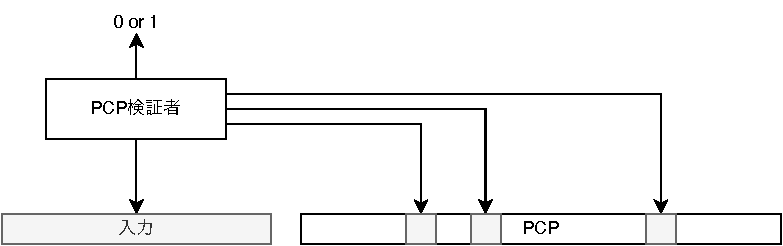
\includegraphics[width=0.8\textwidth]{images/PCPverifier.drawio.pdf}
  \caption{確率的検証可能な証明の概念図. 検証者は乱数を用いて証明$\pi$のうちの一部の文字のみを読み, それに基づいて判定を行う.}
  \label{fig:pcpverifier}
\end{figure}


\begin{definition}{確率的検証可能な証明}{PCP}
  二つの関数$r,q\colon\Nat\to\Nat$に対し, $\PCP(r,q)$を以下の性質を持つ判定集合$L$の集合とする: ある多項式時間オラクル乱択アルゴリズム$V$が存在して, 任意の$x\in\binset^*$に対し,
  \begin{enumerate}
  \item もし$x\in L$ならば, ある$\pi\in\binset^*$が存在して, ($V$の乱択に関して)確率$1$で$V^\pi(x)=1$となる (\emph{完全性}).
  \item もし$x\notin L$ならば, 全ての$\pi\in\binset^*$に対して, ($V$の乱択に関して)確率$1/3$以上で$V^\pi(x)=0$となる (\emph{健全性}).
  \item さらに, 入力長が$n=\abs{x}$のとき, $V^\pi(x)$はオラクル$\pi$のうち高々$q(n)$個の文字を読み, そのランダムシード長は$r(n)$で抑えられる.
  \end{enumerate}
  このようなオラクル乱択アルゴリズム$V$を\emph{PCP検証者}といい, 証明$\pi$を\emph{PCP}という.
\end{definition}
\begin{remark}{PCPの長さ}{PCP-length}
  $\PCP(r,q)$の証明$\pi$の長さは$q(n)2^{r(n)}$で抑えられる.
  各ランダムシード$s \in \binset^{r(n)}$に対して検証者は$\pi$のうち高々$q(n)$個の文字を読むため, 全てのランダムシードを列挙すると, アクセスされる可能性のある$\pi$の文字数は高々$q(n)2^{r(n)}$で抑えられる.
\end{remark}

一般にランダムシード長$r(n)$と読み込む文字数$q(n)$が小さいほど良いPCP検証者であると考えられる.
PCP検証者の構成は非常に難しい.
例えば\cref{ex:graph-coloring-problem}のグラフ彩色問題に対する次の検証者を考えてみよう:
入力としてグラフ$G=(V,E)$と証明として関数$\pi\colon V\to[k]$を受け取り, この関数$\pi$が実際に$G$の$k$-彩色であるかどうかを判定する.
検証者は$G$の辺$\{u,v\}\in E$をランダムに一つ選び, $\pi(u)\neq \pi(v)$であるかどうかによって判定する.
この検証者は$\pi$のうち高々$q(n)=O(1)$個の文字を読み, そのランダムシード長は$r(n)=O(\log n)$で抑えられる.
しかし, この検証者は健全性の条件を満たさない.
実際, $G$が$k$-彩色可能でない場合, どのような関数$\pi\colon V \to [k]$を与えても, 少なくとも一つの辺$\{u,v\}\in E$が存在して$\pi(u)=\pi(v)$となるが, 検証者がこのような辺を引き当てる確率は最悪の場合, $1/\abs{E}$となるからである.

PCP定理とは, ある$r(n)=O(\log n)$, $q(n)=O(1)$に対して$\PCP(r,q)=\NP$が成り立つことを主張する定理である.
例えばグラフ彩色問題は$\NP$に属するため, 実は全段落の$r(n),q(n)$を達成するPCP検証者が存在するのである!

\begin{theorem}{PCP定理}{PCPtheorem}
  ある$r(n)=O(\log n)$, $q(n)=O(1)$に対して$\PCP(r,q)=\NP$が成り立つ.
\end{theorem}

\begin{remark}{片側の包含関係}{one-sided-inclusion}
  PCP定理において, $\PCP(r,q)\subseteq \NP$は容易に示すことができる.
  実際, \cref{rem:PCP-length}により, 証明$\pi$の長さは$q(n)2^{r(n)} = n^{O(1)}$で抑えられる.
  また, $r(n)=O(\log n)$より, 検証者は$2^{r(n)}=n^{O(1)}$個のランダムシードを列挙し, それら全てに対してPCP検証者を適用し, その出力値の多数決をとることで, 入力$x$に対して$x\in L$かどうかを多項式時間で判定できる.
  PCP定理の証明の本質的な難しさは逆側の包含関係$\NP\subseteq \PCP(r,q)$の証明にある.
\end{remark}

\subsection{NP完全性とCook-Levinの定理}

クラス$\NP$に属する全ての問題に対しそれ以上に難しいという性質を\emph{NP困難性}という.
そしてNPに属する問題がNP困難であるとき, その問題は\emph{NP完全}であるという.
ここでは判定問題\footnote{文脈によっては最適化問題や数え上げ問題といった, 判定問題ではない問題に対してもNP困難性の概念が自然に定義されることもあり, この講義でもPCP定理の応用を紹介する際に「最適化問題XはNP困難である」という言い方を用いる箇所がある. その際は最適化問題Xを解く多項式時間アルゴリズムを用いると全てのNPに属する問題が多項式時間で解けるということを意味する.}に対してNP困難性とNP完全性の定義を与える.

\begin{definition}{NP完全性}{NP-complete}
  判定問題$L\in \NP$は, 任意の$L'\in\NP$に対して以下を満たす決定的多項式時間アルゴリズム$A$が存在するとき, \emph{NP完全}であるという ($A$は$L'$に依存してよい):
  文字列$x\in\binset^*$を入力として受け取ったアルゴリズム$A$の出力を$A(x)\in\binset^*$とする.
  このとき, 任意の$x\in\binset^*$に対して, $x\in L'$と$A(x)\in L$は同値である.
  また, このようなアルゴリズム$A$を$L'$から$L$への\emph{カープ帰着}という.
\end{definition}

\begin{remark}{「NP以上に難しい」の意味}{NP-hardness-property}
NP完全な判定問題$L$を解く多項式時間アルゴリズム$A_0$が存在するならば, 任意の$L'\in \NP$に対し$L'$を解く多項式時間アルゴリズムが存在する.
実際, $L'$から$L$へのカープ帰着を$A$とすると, 与えられた$x\in\binset^*$が$x\in L$かどうかはまず, $y=A(x)$を計算し, その後$A_0(y)$を計算することで判定できる.
この意味で$L$は$L'$以上に難しいといえる.

しかし, 二つの問題の困難性を比較する際は必ずしもカープ帰着に拘る必要はない.
実際, 上述のアルゴリズムは$L$を解くアルゴリズム$A_0$を一度だけ用いてしかもその出力$A_0(y)\in\binset$がそのまま$x\in L'$かどうかの答えと一致しているが, 「$L$が解けたら$L'$も解ける」ということを示すのであれば複数の入力$y_1,\dots,y_m$に対して$A_0(y_1),\dots,A_0(y_m)$を計算してもよいし, それらの出力を組み合わせて$x\in L'$かどうかを判定してもよい.
このような自由度の高い操作を許しつつ$A_0$が多項式時間で動くならば全体も多項式時間で動くことが保証されるような帰着を\emph{チューリング帰着}という.
\end{remark}

具体的にカープ帰着含めNP完全性の枠組みが確立されたのは\citet{Karp1972}であるが,
実はそれ以前の\citet{Cook1971}は, カープ帰着とは少し異なる帰着を用いて\emph{回路充足可能性判定問題}と呼ばれる問題がNP完全であることを示していた. 
回路充足可能性判定問題は論理回路に関する問題であり一見するとグラフなどとは関係なさそうに見えるが,
\citet{Karp1972}は, カープ帰着の下でも\cite{Cook1971}の証明は成立することを利用して最大クリーク問題, ハミルトン閉路問題, 彩色数の計算, ナップザック問題といった様々な自然な組合せ最適化問題のNP困難性を証明していった.
\citet{Karp1972}がNP完全性を示したこれらの問題は現在では\emph{Karpの21のNP完全問題} (Karp's 21 NP-complete problems)と呼ばれており,
この成果によってCookは1982年とKarpは1985年にそれぞれチューリング章を受賞している.
また, 実は\citet{Levin1973}も同様の結果を独立に示していたことが判明し(論文の発行当時は冷戦下であったことが災いして違いの認識が遅れてしまった), Levinは2012年にクヌース章を受賞している.
このことから以下に定める回路充足可能性判定問題のNP完全性を示す定理を\emph{Cook-Levinの定理}といい,
この定理は全てのNP完全性の理論の基礎となる計算量理論における最も重要な定理の一つである.

\begin{theorem}{Cook-Levinの定理}{Cook-Levin}
  論理回路$C\colon\binset^n\to\binset$を入力として受け取り, $C(x)=1$を満たす$x\in\binset^n$が存在するかどうかを判定する問題を\emph{回路充足可能性判定問題}(Circuit SAT; circuit satisfiability problem)という.
  回路充足可能性判定問題はNP完全である.
\end{theorem}

Cook-Levinの定理の証明はクラスNPの検証者を非決定的チューリング機械で模倣し, その機械を回路として表現することによって与えられる.
すなわち, 回路による計算はチューリング機械を模倣できるという性質が完全性において肝要な性質であり, 以下のように述べられる:
\begin{claim}{チューリング機械を模倣する回路}{Turing-machine-circuit}
  任意の多項式時間チューリング機械$M$に対して, ある回路族$(C_n)_{n\in\Nat}$が存在して以下が成り立つ:
  \begin{itemize}
    \item 全ての$n\in\Nat$に対して, $C_n\colon\binset^n\to\binset$は$n^{O(1)}$個のゲート(AND,OR,NOT)を含む. なお, ここでは全ての素子は二つの入力を受け取り一つの出力を持つ.
    \item 任意の$n\in\Nat$と全ての$x\in\binset^n$に対し, $M$が$x$を受理することと$C_n(x)=1$は同値.
    \item 各$C_n$は$n^{O(1)}$時間で構成できる.
  \end{itemize}
\end{claim}
\cref{claim:Turing-machine-circuit}を証明するにはチューリング機械の厳密な定義なども必要であり講義では詳しくは扱わないが, その概要を以下に説明する.
\begin{proof}[証明の概要.]
  チューリング機械とは, 無限の長さの\emph{記憶テープ}を備えた有限状態機械である.
  \emph{記憶テープ}とは無限の長さの記号列であり, 入力$x\in\binset^*$に対して
  まずは最初の$\abs{x}$文字は$x$が記載されており, それ以外の文字は全て$\bot$(空白であることを表す記号)である.
  また, \emph{ヘッド}と呼ばれるポインタがあり, これは現在は記憶テープのどの位置の文字を読み書きするかを表す.
  各ステップにおいて, 現在の状態とヘッドが指し示す文字を参照し, 次の状態, 現在のヘッドに書き込む内容, ヘッドの移動方向(左右もしくはそのまま)を決める.
  さらに機械には二つの相異なる二つの特別な状態$q_{\mathrm{accept}}$と$q_{\mathrm{reject}}$があり, これらに遷移すると計算が終了する. 終了時の状態に応じてチューリング機械の出力(acceptまたはreject)が決まる.
  
  \begin{figure}[ht]
    \centering
    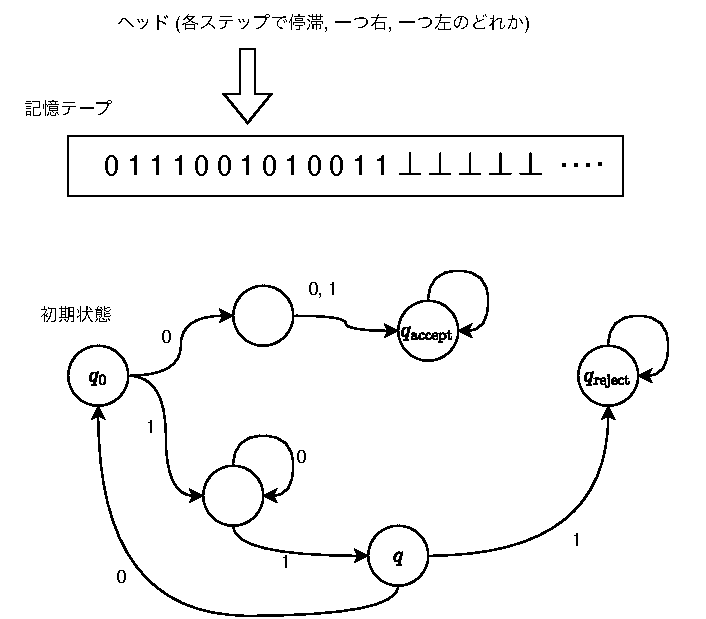
\includegraphics[width=0.8\textwidth]{images/Turing.pdf}
    \caption{チューリング機械の一例. 各状態において, ヘッドの指し示す記憶テープの値のラベルがついた有効辺に沿って遷移し, そのヘッドの位置にある記憶テープの値を必要があれば書き換え, 最後にヘッドの位置を一つ右, 一つ左のいずれかに移動するかそのままにする.}
  \end{figure}
  
  計算が終了するまでに要したステップ数をこのチューリング機械の\emph{(時間)計算量}という.
  チューリング機械$M$が多項式時間であったとする. このとき, 任意の十分大きな$n\in\Nat$と任意の$x\in\binset^n$に対して, $M$の計算の任意の時点での記憶テープの内容($\bot$以外の文字の個数)は高々$n^{O(1)}$文字で表現できる.
  また, ヘッドの指し示す位置は$O(\log n)$ビットで表現でき, 状態の個数は高々$O(1)$である.
  従って, 任意の時点でのチューリング機械の, 記憶テープの内容も含めた状態(便宜上これを計算状態と呼ぶことにする)は高々$n^{O(1)}$ビットで表現できる.
  また, 記憶テープの書き換えは高々$1$ビットの書き換えであり, ヘッド位置の変更も加算と減算で計算できるため,
  チューリング機械の計算の各ステップもまた小さいサイズの回路によって模倣できる. すなわち, 現在の計算状態を入力として受け取り, 計算状態の第$i$番目のビットを出力する回路$C_i$を用意してこれを全ての$i\in[n^{O(1)}]$に対して並べることによって, 回路として表現できる.
  これを全てのステップについて並べれば, チューリング機械$M$を模倣する多項式サイズの回路$C$ (すなわち, $M(x)$の最終状態が$q_{\mathrm{accept}}$または$q_{\mathrm{reject}}$であるかどうかを判定する回路)が得られる.
\end{proof}

これを用いてCook-Levinの定理の証明を与える.

\begin{proof}[\cref{thm:Cook-Levin}の証明]
  NPの定義より, 任意の判定問題$L\in\NP$に対して, 多項式時間のNP検証者$V(x;\pi)$が存在する.
  \cref{claim:Turing-machine-circuit}より, このNP検証者を模倣する回路族$(C_n)_{n\in\Nat}$が存在する.
  特に, 入力$x\in\binset^*$が与えられたとき, $V(x;\cdot)$というチューリング機械を模倣する回路$C_x\colon\binset^{\abs{\pi}}\to\binset$が多項式時間で構成できる.
  さらにこれが$L$から回路充足可能性判定問題へのカープ帰着になっていることを確認すれば証明は完了する.
  実際, $x$がYesインスタンスであるならば$V(x;\pi)=1$を満たす$\pi$が存在することから, $C_x$は充足可能である.
  一方で$x$がNoインスタンスであるならば$C_x$は充足可能でない.
  従って$x\mapsto C_x$は確かに$L$から回路充足可能性判定問題へのカープ帰着になっている.
\end{proof}

Cook-Levinの定理を用いると, 以下に示す二次方程式系の充足可能性判定問題がNP完全であることが示せる:
\begin{theorem}{二次方程式系の充足可能性判定問題}{ThreeQuadEQ-NP-complete}
  判定問題$\QuadEQ$を以下のように定義する:
  $m$個の$n$変数二次関数$f_1,\dots,f_m\colon \F^n\to\F_2$が与えられる.
  このとき, ある$x\in\F^n$が存在して$f_1(x)=\dots=f_m(x)=0$を満たすかどうかを判定せよ.
  特に, 全ての$i\in[m]$に対し, $f_i(x_1,\dots,x_n)$の値が高々$k$個の変数$x_{i_1},\dots,x_{i_k}$の値のみに依存するようなとき, $k$-$\QuadEQ$と呼ぶ.
  
  $\ThreeQuadEQ$はNP完全である.
\end{theorem}
\begin{proof}
  $\ThreeQuadEQ$はNPに属する.
  実際, NP証拠として連立方程式の解$x\in\F^n$を与え, それが実際に$f_1(x)=\dots=f_m(x)=0$を満たすかどうかは$n^{O(1)}$時間で判定できる (入力として$f_1,\dots,f_m$が与えているため, これを二進文字列として表現したときの長さは$n$以上である).

  次に, 回路充足可能性判定問題から$\ThreeQuadEQ$へのカープ帰着を構成する.
  回路充足可能性判定問題の入力$C\colon\binset^n\to\binset$が与えられたとき, これらの変数を$x_1,\dots,x_n$とする.
  各ゲートに対し, そのゲートに対応する変数を新たに用意し, これらを$x_{n+1},\dots,x_{n+s}$とする ($s$は回路$C$に含まれる入力以外のゲートの個数).
  各$k\in[s]$に対し, 変数$x_{n+k}$に対応するゲート$c$の入力に対応する変数を$x_i,x_j$とし (もしもゲートがnotゲートであったならば$x_i$のみを考える), さらに$i,j < n+k$を満たすとする (こうなるように, 入力$x$に近い順にゲートの番号づけを行う).
  関数$f_k\colon \F^n\to\F_2$を以下のように定義する: $k\in[s]$に対し
  \begin{align*}
    f_k(x) = \begin{cases}
      x_k - x_i x_j & \text{if ゲート$c$がANDゲート}, \\
      x_k - (x_i + x_j - x_i x_j) & \text{if ゲート$c$がORゲート}, \\
      x_k - (1-x_i) & \text{if ゲート$c$がNOTゲート}.
    \end{cases}
  \end{align*}
  $k=s+1$に対して$f_{s+1}(x) = 1 - x_{n+s}$と定義する (\cref{fig:circuit-to-3-QUADEQ}を参照).
  このとき, 各$f_k$は高々三つの変数にのみ依存するため,
  $(f_k)_{k\in[s+1]}$は$\ThreeQuadEQ$のインスタンスとなり, 回路$C$が入力として与えられたとき多項式時間で構成できる.

  \begin{figure}[ht]
    \centering
    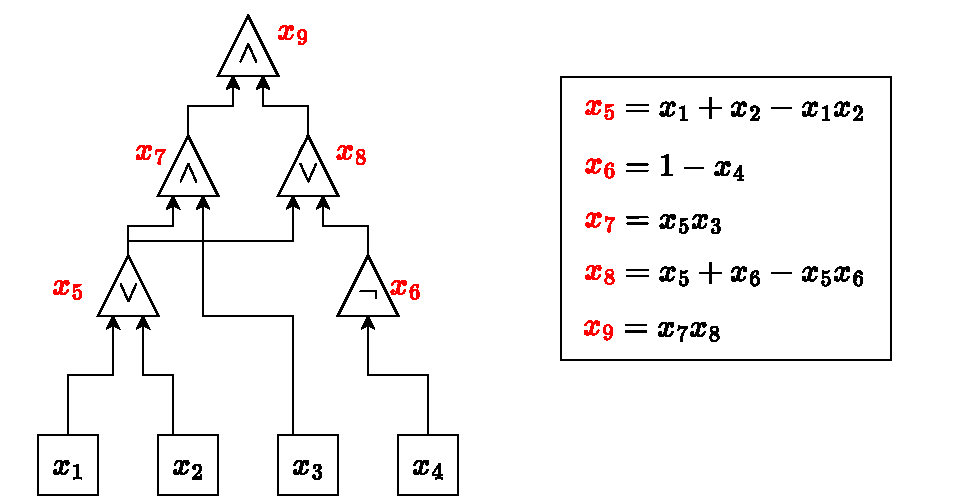
\includegraphics[width=0.8\textwidth]{images/circuit_to_3-QUADEQ.pdf}
    \caption{回路充足可能性判定問題から$\ThreeQuadEQ$へのカープ帰着の例. $(\text{左辺})-(\text{右辺})$が各$f_k$となる. \label{fig:circuit-to-3-QUADEQ}}
  \end{figure}

  最後に$C$が回路充足可能性判定問題のYesインスタンスであることと$(f_k)_{k\in[s+1]}$が$\ThreeQuadEQ$のYesインスタンスであることが同値であることを示す.
  識別のため, $C$の入力は$x\in\binset^n$とし, $f_k$の入力は$\overline{x} \in \binset^{n+s}$とする.
  まず, $C$がYesインスタンスであるとき, ある$x\in\binset^n$が存在して$C(x)=1$を満たす.
  出力値$C(x)$を計算するときの途中の各ゲートの出力値をそのまま対応する変数に割り当てることによって$\overline{x}$を構成すると, 確かに全ての$k$に対して$f_k(\overline{x})=0$を満たす.
  一方, $(f_k)$がYesインスタンスであるとき, 最初の$x=(\overline{x}_1,\dots,\overline{x}_{n})$とすれば, $C(x)=1$となる.
  従って, $C\mapsto (f_k)_{k\in[s+1]}$は確かに回路充足可能性判定問題から$\ThreeQuadEQ$へのカープ帰着になっている.
\end{proof}

Cook-Levinの定理を用いると3彩色問題$\ThreeCOL$のNP完全性を示すことができる.
具体的には3-SATと呼ばれるNP完全な問題を$\ThreeCOL$に帰着させることで$\ThreeCOL$のNP完全性を示せる (本講義では割愛).

\begin{theorem}{3彩色問題のNP完全性}{3-coloring-problem-NP-complete}
  3彩色問題$\ThreeCOL$はNP完全である. すなわち, 任意の$L\in\NP$に対して, 多項式時間アルゴリズム$f$が存在して, 任意の$x\in\binset^*$に対して$x\in L$と$f(x)\in\ThreeCOL$は同値である.
\end{theorem}

\cref{thm:3-coloring-problem-NP-complete}により, PCP定理を証明するには, $\ThreeCOL$に対する効率的なPCP検証者を構成すればよいことがわかる.

\begin{theorem}{3彩色問題のPCP検証者}{3-coloring-problem-PCP-verifier}
  ある$r(n)=O(\log n),q(n)=O(1)$に対して, 3彩色問題$\ThreeCOL$は$\PCP(r,q)$に属する.
\end{theorem}

\begin{exercise}{}{exercise2}
  \cref{thm:3-coloring-problem-PCP-verifier,thm:3-coloring-problem-NP-complete}を仮定して, PCP定理(\cref{thm:PCPtheorem})を証明せよ.
\end{exercise}

\section{PCP定理の応用}
PCP定理の応用として, 様々な組合せ最適化問題に対する近似のNP困難性を導出することができる.

\section{PCP定理の背景}
PCP定理は組合せ最適化の分野への著しい応用を持つため,
その視点からPCP定理を紹介する文献ではなぜPCP定理が発見されたのかという動機が語られることが少ないように思われる.
そこで, この節ではPCPという計算量クラスを考えるに至った背景について軽く触れたい.
PCP定理は1992年にAroraとSafraによって証明された.
その後, 2005年にDinurによって証明が簡略化され, 2010年にAroraとBarakによって証明が再構成された.


